\section{Requisitos}
\label{sec:requisitos}
\subsection{Requisitos Funcionais}

\begin{itemize}
\item Simular corrida de bicicleta em ambiente virtual.
\item Manter dados do usuário.
\item Visualizar dados de desempenho.
\item Gerar energia que alimente pelo menos parcialmente o sistema.
\item Monitorar movimentação da bicicleta.
\item Monitorar os dados fisiólogicos do usuário de respiração, batimentos cardiacos e resistência galvânica da pele.
\item Trasmitir dados monitorados para o óculos.
\item Controlar atuadores para emular movimentos do ambiente de realidade virtual.
\item Projeto de uma estrutura adaptável que comporte bicicletas de aros de 26 ou 29 polegadas.
\item Projeto de uma estrutura que comporte sensores, motores e aparatos tecnológicos.

\end{itemize}

\subsection{Requisitos de Desempenho}

\begin{itemize}
\item O jogo deve executar a uma taxa mínima de 24 frames por segundo.
\item O jogo deve responder às entradas dos outros sistemas a um tempo de 100 milissegundos.
\item O jogo deverá ser disponível para os sistemas operacionais \textit{Windows} e \textit{Linux}.
\item O sistema de alimentação deve fornecer uma autonomia mínima de 5 minutos para o sistema.
\item O sistema de controle de carga deve ser sincronizado com a realidade do jogo. 
\item Os sistemas de monitoramento do atleta devem ser enviados via \textit{wireless}.
\item Os sistemas de monitoramento devem ser construídos com robustez suficiente de maneira que possam ser instalados em luvas, pulseiras, cintos e/ou coletes para que possam ser usados pelo usuário e estar em constante movimento.
\item Permitir movimentação do guidão da bicicleta.
\item Ser firme e segura a fim de prevenir acidentes por tontura ou erro na simulação.
\end{itemize}

%\subsection{Requisios Estatuários}

\section{Estudo da Viabilidade do Projeto}

\subsection{Infra-estrutura}

	O espaço disposto para o projeto é o Laboratório de Pesquisa em Artes e TecnoCiência (LART) localizado dentro do MOCAP. Este laboratório visa integrar artistas e cientistas em uma visão mais humanista dos avanços tecnológicos.
Ele nos promove um espaço de trabalho, peças, computadores e apoio dos professores.
Ainda temos como espaço de trabalho o Galpão da FGA, onde temos uma série de máquinas e técnicos para a produção da estrutura da plataforma.

\subsection{Viabilidade Técnica}
	
	O produto é uma plataforma de realidade virtual na qual insere-se uma bicicleta. Esse é um produto que está disponível no mercado com diversas tecnologias e formas possíveis por empresas pioneiras, como por exemplo a WideRun, a Zwift e a VirZOOM. A plataforma será capaz de gerar, por óculos de realidade virtual, um ambiente, e haverá toda a aquisição de dados por meio de sensores espalhados pela bicicleta, a fim de monitorar a atividade física exercida pelo usuário. Há mais de uma década que diversos artigos científicos mostram os resultados de estudos do comportamento fisiológico em ambiente virtual \cite{plante} \cite{mestre} \cite{chihak} mostrando a necessidade e interesse neste tópico. Nossa solução ainda permite a economia de energia, tendo em vista que parte do sistema é um microgerador de energia, com o intuito de fornecer energia para os componentes do sistema, algo também que esta começando a se espalhar em academias e projetos de pesquisas.
    	
	O objetivo desta plataforma é estudar e monitorar os ciclistas enquanto realizam exercício indoor em um ambiente virtual, uma área inovadora que tem ainda muito a avançar, tanto em pesquisas quanto em mercado e em implementação de recursos tecnológicos, tais como sensores de frequência cardíaca, microgeração de energia e imersão em realidade virtual, os quais são novidades para boa parte da população. Tais estudos serão conduzidos pelo LART, que se beneficiará dessa plataforma de baixo custo de ciclismo e óculos de realidade virtual, para fazer essas pesquisas de ponta.

\subsubsection{Investimentos fixos programados} 
	Há a disponibilidade de local físico para trabalho, o LART, portanto, despreza-se os custos com instalações complementares. Os equipamentos principais a serem utilizados, tais como o \textit{Oculus Rift}, estão sendo disponibilizados também pelo laboratório. Os custos fixos programados seriam apenas com compras de componentes para a instrumentação e controle ativo da plataforma e para a construção da estrutura da plataforma.

\subsection{Aspectos Organizacionais e de Gestão}
	
	O projeto é desenvolvido por alunos de Engenharias (Aeroespacial, Automotiva, Eletrônica, Energia e Software), apoiado por professores gabaritados em gestão de projetos e com experiência em lecionar a matéria de Projeto Integrador em Engenharia II. Haverão pontos de controle pré-definidos por estes professores que irão servir de avaliação e acompanhamento do projeto, contudo, a equipe se propõe a elaborar um cronograma com datas específicas de construção, validação e conclusão dos subsistemas.
    
	Dos membros da equipe, todos estão no final do curso, o que os deixa em posição de conseguirem construir cada subsistema do projeto. Ainda temos alguns alunos de eletrônica e software com experiência em realidade virtual, alunos de automotiva experientes em design, simulação e fabricação, alunos de software premiados em competição.
	
\subsection{Planejamento Estratégico}

\begin{table}[!ht]
\centering
\caption{Matriz S.W.O.T.}
\label{swot}
\begin{tabular}{|l|l|l|}
\hline
              & \textbf{Fatores Controláveis }                                                                                                                             & \textbf{Fatores Externos}                                                                                                                                \\ \hline
\textbf{Pontos Fortes} & \begin{tabular}[c]{@{}l@{}}Alunos de \\várias engenharias;\\ É um projeto simples\\que pode ser ampliado;\\ Tema instigante e inovador.\end{tabular} & \begin{tabular}[c]{@{}l@{}}Apoio do LART;\\ Suporte financeiro de professores;\\ Atuadores D-Box a disposição;\\ Acesso ao Galpão.\end{tabular} \\ \hline
\textbf{Pontos Fracos} & \begin{tabular}[c]{@{}l@{}}Desconhecimento inicial \\de algumas tecnologias \\chave para o projeto;\\ Tempo bem curto.\end{tabular}                   & \begin{tabular}[c]{@{}l@{}}Greve;\\ Quebrar algum equipamento essencial.\end{tabular}                                                           \\ \hline
\end{tabular}
\end{table}

	Com base na pesquisa de tendências já realizada, em todo o trabalho já feito e na matriz S.W.O.T. o projeto inicial será o cenário mais simples possível com as exigências de mais alto nível. Esse cenário será adaptável a melhorias que imagina-se serem possíveis, porém não há garantia de tempo hábil. Assim, caso o projeto básico termine antes do previsto, acrescentar-se-á algumas funções que seriam facilmente implementadas no design inicial.

	Um exemplo claro disso é a utilização de atuadores para a inclinação da plataforma. Isso deixaria a simulação mais real, porém não se sabe se haverá tempo suficiente. Para tanto, projetar-se-á a plataforma que possa ser facilmente integrada com uma base de atuadores D-Box, que já consta no LART. Mas antes disso, tem que se assegurar que todos os demais requisitos do projeto estejam funcionando. Uma descrição detalhada dos requisitos da plataforma se encontram na seção~\ref{sec:requisitos}.

	Assim, os requisitos iniciais visarão segurança do usuário em caso de tontura, dificuldade de pedalada em simulação de subida, geração de energia a partir da movimentação da bicicleta e criação de ambiente virtual integrado com a plataforma real.

	Esses objetivos primários foram discutidos com os professores do LART e com os orientadores da disciplina e acredita-se que sejam factíveis e que são o mínimo esperado pelo grupo.


\section{Escopo}
\subsection{Definição do Escopo}

A proposta do projeto é composto pela plataforma estática iterativa, a imersão em ambiente de realidade virtual e a medição de dados fisiológicos e de desempenho.

A plataforma estática deve ser de tal forma que o usuário tenha como treinar e sentir resultados assim como na corrida em ambiente livre. Para isso a estrutura tem um projeto que permite o usuário acoplar sua própria bicicleta para desenvolver suas atividades e permitir que os atuadores possam oferecer uma resposta de maneira similar para eventos comuns a uma corrida de bicicleta, tais como subida, descida, vibração e aceleração.

O ambiente em realidade virtual será desenvolvido visando a criação de um jogo a ser executado em um \textit{Oculus Rift} padrão. Este tipo de óculos é uma ferramenta usada para promover imersão do usuário em um cenário de realidade virtual 3D e seu objetivo é atuar em sincronia com a plataforma estática proporcionando todo o estímulo visual do trajeto de corrida.

Os sistemas de monitoramento irão colher diversos dados do usuário e da própria bicicleta e armazenar os mesmos, para que possam ser observados em tempo real pelo usuário ou ainda ser expostos a uma na análise posterior a execução.

O intuito destas três abordagens é permitir que o usuário tenha a opção de praticar sua rotina de atividades, com sua própria bicicleta, em um ponto estático e possa ter uma métrica desta execução.

\subsection{Processo de Formalização de Aprovação}

A fim de conseguir controlar as entregas foi definido um processo sob a qual toda atividade que resulte em algo entregável deve passar. 

Os objetivos do processo consistem em verificar se aquele entregável foi submetido a um conjunto de testes e se ele propicia alguma alteração no escopo. Para tanto, segue o processo juntamente com a descrição das atividades:

 \begin{center}
	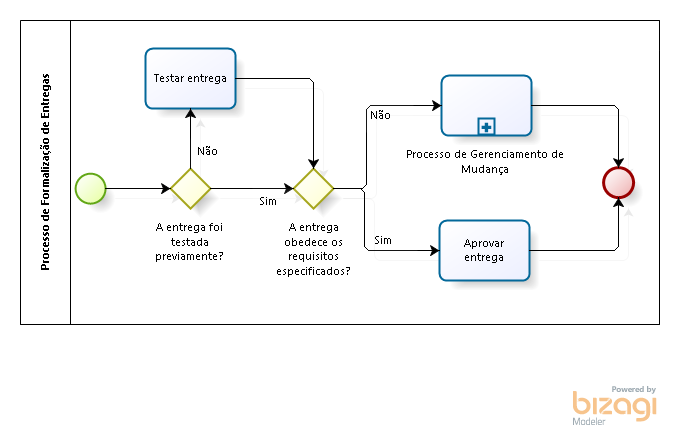
\includegraphics[scale=0.9]{figuras/formalizacaoentregas}
	\captionof{figure}{Processo de Formalização de Entregas.}
\end{center} 

\begin{itemize}
\item \textbf{Testar entrega}
Consiste na avaliação do que foi produzido, com o intuito de garantir que está pronto para ser utilizado. Uma prática importante é validar os pontos de extremidade que possam vir a ocorrer com o construido.

\item \textbf{Processo de Gerenciamento de Mudança}
Uma vez que está sendo entregue pode afetar diretamente o planejamento, foi definido um processo de gerenciamento de mudança, que é melhor explicado na próxima subseção.

\item \textbf{Aprovar entrega}
Estando testado e verificado que a entrega obedece aos requisitos especificados, ela é dita como aprovada. Aprovar a entrega consiste em atualizar o \textit{status} do que faz referência a ela, como o cronograma. 
\end{itemize}

\subsection{Processo de Gerenciamento de Mudança}

Toda vez que o escopo necessitar de uma alteração, devem ser realizadas as atividades do processo de gerenciamento de mudança do escopo que está descrito no diagrama da figura \textcolor{blue}{3}.

\begin{center}
	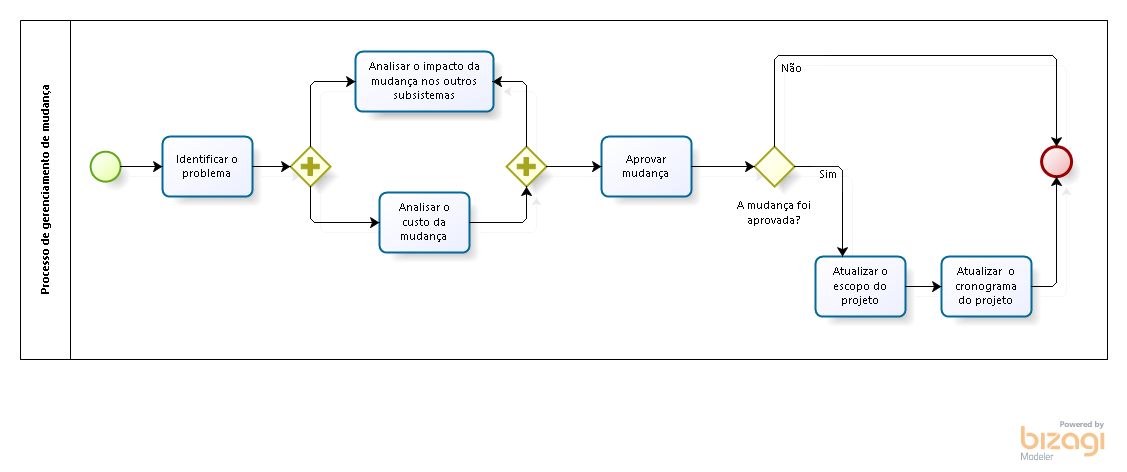
\includegraphics[scale=0.5]{figuras/mudancapi2}
	\captionof{figure}{Processo de Gerenciamento de Blocos.}
\end{center} 

As atividades do processo de gereciamento de mudança são:
 
\begin{itemize}

\item \textbf{Identificar o Problema}
Nesta atividade, a equipe deve identificar o problema que ocasionou a mudança do escopo. O resultado desta atividade facilitará as análises posteriores do processo.

\item \textbf{Analisar o impacto da mudança nos outros subsistemas}
A partir da identificação do problema, a equipe deve analisar o impacto desta mudança nos outros subsistemas. Tudo o que deverá ser implementado no projeto devido à mudança solicitada é identificado e analisado nesta atividade.

\item \textbf{Analisar o custo da mudança}
A equipe deve analisar o custo que a mudança solicitada vai gerar ao projeto.

\item\textbf{ Aprovar mudança}
Após a análise de impacto e custo no projeto, a equipe deve acordar se a mudança será realmente encorporada no projeto ou não, caso os impactos e os custos sejam prejudiciais.

\item \textbf{Atualizar o escopo do projeto}
O escopo do projeto deve ser atualizado com todas as mudanças identificadas na atividade de Analisar o impacto da mudança nos outros subsistemas.

\item \textbf{Atualizar o cronograma do projeto}
O cronograma deve ser adaptado com as mudanças encorporadas a fim de atender o prazo estabelicido do projeto.

\end{itemize}

\section{Análise Crítica de Projeto e Desenvolvimento}

\subsection{Processo de Gerenciamento dos Riscos}

O principal objetivo do processo de gerenciamento dos riscos é minimizar e controlar os eventuais impedimentos que ocorram no projeto e explorar os acontecimentos positivos. Em geral, neste processo são identificados todos os riscos de todas as categorias possíveis, cujo são analisados e respostas à eles caso ocorram são planejadas. As atividades do processo de gerenciamento de riscos estão descritas abaixo.

\begin{center}
	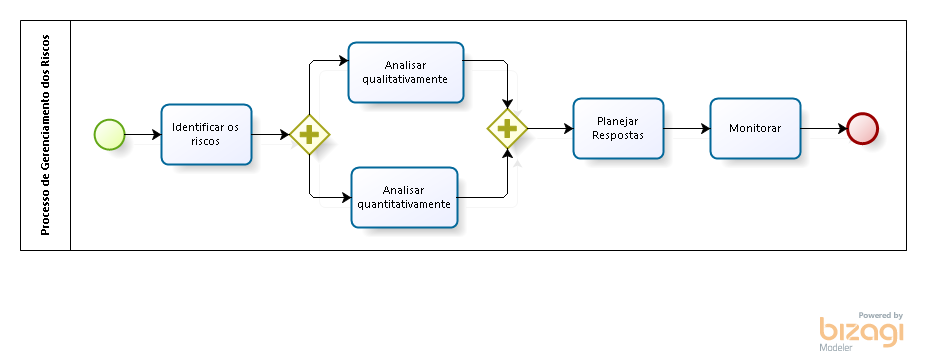
\includegraphics[scale=0.7]{figuras/riscos}
	\captionof{figure}{Processo de Gerenciamento de Riscos.}
\end{center} 

\begin{itemize}
\item \textbf{Identificar riscos:}
Consiste em elencar os riscos que podem afetar o desenvolver do projeto. Além de listá-los procura-se entender algumas de suas características para que sejam analisadas posteriormente.
\item \textbf{Analisar qualitativamente:}
Nesta etapa são aplicadas métricas de impacto e probabilidade aos riscos a fim de obter uma compreensão maior sobre eles.
\item \textbf{Analisar quantitativamente:}
Consiste em analisar de forma numérica os riscos para investigar melhor as métricas definidas no processo anterior.
\item\textbf{Planejar respostas:}
Com base na análise feita, é estipulado um conjunto de ações a serem tomadas de acordo com cada risco.
\item \textbf{Monitorar:}
Consiste em controlar os riscos durante o projeto, avaliando as suas causas, e executando as ações planejadas.
\end{itemize}

\subsection{Categoria dos Riscos}
Analisando a natureza dos riscos, os mesmos foram categorizados em três principais tipos:

\begin{itemize}
\item \textbf{Riscos Externos}: acontecimentos inerentes ao projeto que impactam no planejamento e desenvolvimento do mesmo. Como por exemplo, a falta de financiamento dos patrocinadores.
\item \textbf{Riscos Técnicos:} eventos intrinsecamente ligados com a construção do produto. Um exemplo que pode ser citado é a descontinuação das tecnologias que serão utilizadas.
\item \textbf{Riscos Gerencias:} estão relacionados ao mau planejamento e controle do projeto ocasionando impactos no produto final. Citando caso análogo, a definição de um escopo muito grande para o prazo de tempo do projeto.
\end{itemize}

\subsection{Definições de Probabilidade e Impacto dos Riscos}

Abaixo segue um conjunto de pesos da probabilidade e do impacto. Tais valores servirão de base para a priorização dos riscos, a fim de que ganhem um maior controle do que os outros.

\subsubsection{Probabilidade}

\begin{table}[h]
\centering
\caption{Probabilidade}
\label{probabilidade}
\begin{tabular}{|l|l|l|}
\hline
\textbf{Probabilidade (P)} & \textbf{Intervalo} & \textbf{Peso}\\  \hline
Muito Baixa       & 0 \textless= P \textless=20\%     & 1    \\
Baixa             & 20\% \textless P \textless= 40\%  & 2    \\
Moderada          & 40\% \textless P \textless= 60\%  & 3    \\ 
Alta              & 60\% \textless P \textless= 80\%  & 4    \\ 
Muito Alta        & 80\% \textless P \textless= 100\% & 5    \\ 
\hline
\end{tabular}
\end{table}

\subsubsection{Impacto}

\begin{table}[h]
\centering
\caption{Impacto}
\label{impacto}
\begin{tabular}{|l|l|l|}
\hline
\textbf{Impacto (I)} & \textbf{Descrição}                                & \textbf{Peso} \\  \hline
Muito Baixo          & Quase que imperceptível ao projeto                & 1             \\
Baixo                & Pouca influência no desenvolvimento do projeto    & 2             \\
Moderado             & Notável ao projeto, mas sem grandes consequências & 3             \\
Alto                 & Dificulta o desenvolvimento do projeto            & 4             \\ 
Muito Alto           & Impossibilita o prosseguimento do projeto         & 5             \\ 
\hline
\end{tabular}
\end{table}

\subsection{Matriz de probabilidade e Impacto}

	Os pesos da probabilidade de um evento ocorrer em contraste ao risco que este mesmo oferece é apresentado na tabela \textcolor{blue}{4}.  

\begin{table}[h]
\centering
\caption{Probabilidade e Impacto}
\label{probabilidade-impacto}
\begin{tabular}{|l|l|l|l|l|l|}
\hline
P\textbackslash I  & Muito Baixo & Baixo & Moderado & Alto & Muito Alto \\ \hline
Muito Baixa                  & 1                               & 2                         & 3                   & 4               & 5                     \\ 
Baixa                    & 2                               & 4                         & 6                   & 8               & 10                    \\
Moderada                     & 3                               & 6                         & 9                   & 12              & 15                    \\ 
Alta                         & 4                               & 8                         & 12                  & 16              & 20                    \\ 
Muito Alta                   & 5                               & 10                        & 15                  & 20              & 25                    \\ 
\hline
\end{tabular}
\end{table}

\subsubsection{Prioridade}
Com base na matriz apresentada é possível determina o nível de prioridade de cada risco como consequência dos intervalos definidos.

\begin{table}[h]
\centering
\caption{Prioridade}
\label{prioridade}
\begin{tabular}{|l|l|}
\hline
Prioridade & Intervalo \\ 
\hline
Baixa      & 1-5       \\ 
Média      & 6-15      \\ 
Alta       & 16-25     \\ 
\hline
\end{tabular}
\end{table}

\subsection{Registro dos Riscos}

\subsubsection{Riscos Negativos do Projeto}

\begin{table}[H]
\centering
\caption{Riscos do Projeto}
\label{riscos-negativos-projeto}
\begin{tabular}{|l|l|l|l|}
\hline
\textbf{Causa} & \textbf{Risco} & \textbf{Descrição} & \textbf{Impacto} \\ \hline
Inexperiência da equipe & R01 & \begin{tabular}[c]{@{}l@{}}Dificuldades com as tecno-\\ logias e recursos utilizados\\ para a construção da plata-\\ forma\end{tabular} & \begin{tabular}[c]{@{}l@{}}Produtividade baixa e \\ atraso nas entregas\end{tabular} \\
Escopo mal definido & R02 & Mudança no escopo & \begin{tabular}[c]{@{}l@{}}Replanejamento das\\  atividades\end{tabular} \\
\begin{tabular}[c]{@{}l@{}}Falha no planejamento ou \\ baixa produtividade da \\ equipe ou desmotivação \\ dos integrantes\end{tabular} & R03 & Atraso nas entregas & Atraso no cronograma \\
\begin{tabular}[c]{@{}l@{}}Desmotivação dos inte-\\ grantes\end{tabular} & R04 & \begin{tabular}[c]{@{}l@{}}Membros desistirem da\\  disciplina\end{tabular} & Sobrecarga de trabalho \\
Falha no planejamento & R05 & \begin{tabular}[c]{@{}l@{}}Não concluir o escopo \\ do projeto\end{tabular} & \begin{tabular}[c]{@{}l@{}}O grupo pode ser penali-\\ zado com a nota do tra-\\ balho\end{tabular} \\
\begin{tabular}[c]{@{}l@{}}Professores e/ou técnicos\\  insatisfeitos\end{tabular} & R06 & Greve na universidade & \begin{tabular}[c]{@{}l@{}}Mudança no planejamento \\ e interrupção do projeto\end{tabular} \\
\begin{tabular}[c]{@{}l@{}}Interrupção no financia-\\ mento do projeto\end{tabular} & R07 & \begin{tabular}[c]{@{}l@{}}Desinteresse dos patroci-\\ nadores\end{tabular} & \begin{tabular}[c]{@{}l@{}}Mudança no planejamento \\ financeiro e no orçamento \\ do projeto\end{tabular} \\ \hline
\end{tabular}
\end{table}

\begin{table}[H]
\centering
\caption{Riscos do Projeto Estrutual}
\label{riscos-negativos-estrutura}
\begin{tabular}{|l|l|l|p{5cm}|}
\hline
\textbf{Causa} & \textbf{Risco} & \textbf{Descrição} & \textbf{Impacto} \\ \hline
\begin{tabular}[c]{@{}l@{}}Atraso na entrega \\ da estrutura\end{tabular} & R08 & \begin{tabular}[c]{@{}l@{}}Atraso na produção/monta- \\gem da estrutura no prazo \\ estipulado\end{tabular} & \begin{tabular}[c]{@{}l@{}}Produtividade baixa e \\ atraso nas entregas\end{tabular} \\

\begin{tabular}[c]{@{}l@{}}Técnicos insatisfeitos\end{tabular} & R09 & \begin{tabular}[c]{@{}l@{}}Mau relacionamento com \\os técnicos
\end{tabular} & \begin{tabular}[c]{@{}l@{}}Orçamento maior que o \\necessário e também uma \\ logística mais complexa\end{tabular} \\ 

\begin{tabular}[c]{@{}l@{}}Professores contra\end{tabular} & R10 & \begin{tabular}[c]{@{}l@{}}Um dos fatores estipulados \\por um dos professores pa-\\trocinadores é que o projeto \\ fique na antessala do Mocap; \\tal lugar também é dividido \\entre outros professores e \\estes podem ser contra a a-\\plicação do projeto no local
\end{tabular} & \begin{tabular}[c]{@{}l@{}}Se essa possibilidade ocorrer  \\ ou terá que ser confecciona-\\do uma estrutura fácil de  \\ ser retirada do laboratório \\ ou estipulado outro lugar \\ para a aplicação \end{tabular} \\

\begin{tabular}[c]{@{}l@{}}Professores que dão \\ aula no Mocap incomo- \\ dados com os alunos\end{tabular} & R11 & \begin{tabular}[c]{@{}l@{}}Para entrarem no LART os \\ alunos terão que pedir para \\ que os funcionários abram e \\ fechem as portas \\ e também terão que atra- \\ vessar a aula no momento \\ de aula, assim como conver-\\sas e barulhos de trabalho
\end{tabular} & \begin{tabular}[c]{@{}l@{}}Prejudicará a fluência e li-\\berdade de trabalho. Se fo-\\rem barrados ou alertados \\ pelos professores pelo incó-\\modo tornará mais difícil \\ o trabalho ágil\end{tabular} \\ 

\begin{tabular}[c]{@{}l@{}}Falta de equipamentos \\ e peças\end{tabular} & R12 & \begin{tabular}[c]{@{}l@{}}Falta ou má aplicação dos \\ equipamentos já comprados \\ ou produzidos
\end{tabular} & \begin{tabular}[c]{@{}l@{}}Atraso no cronograma, pois \\ deverá ser fabricado ou en-\\comendado outra peça\end{tabular} \\ 

\begin{tabular}[c]{@{}l@{}}Falta de dinheiro\end{tabular} & R13 & \begin{tabular}[c]{@{}l@{}}Alguns equipamentos e ma-\\ teriais possuem o preço bas-\\ tante alto e contando com o \\ orçamento alto das outras \\ subequipes pode acontecer \\ de ter escassez de financeiro
\end{tabular} & \begin{tabular}[c]{@{}l@{}}Atraso no projeto para en-\\contrar outra possibilidade \\ mais barata ou adaptação \\ do projeto\end{tabular} \\ 

\begin{tabular}[c]{@{}l@{}}Falhas, trincas, desmon- \\ tes no momento da in- \\tegração final\end{tabular} & R14 & \begin{tabular}[c]{@{}l@{}}Após a construção final po-\\de ocorrer falhas na estrutu- \\ra
\end{tabular} & \begin{tabular}[c]{@{}l@{}}Atraso no projeto para a \\ manutenção\end{tabular} \\

\begin{tabular}[c]{@{}l@{}}Danos a patrimônios \\ da UnB\end{tabular} & R15 & \begin{tabular}[c]{@{}l@{}}Danos a patrimônios como:\\ quebra de furadeira, torno,\\ fresa e cnc, furar a lona ca-\\ve ou algum patrimônio no \\ Mocap
\end{tabular} & \begin{tabular}[c]{@{}l@{}}Aumentos do custo do pro-\\jeto\end{tabular} \\ 

\begin{tabular}[c]{@{}l@{}}Geometria incompatível \\ a outro subsistema\end{tabular} & R16 & \begin{tabular}[c]{@{}l@{}}Na integração final pode a-\\contecer que um subsistema \\ tenha projetado de uma for-\\ma que não encaixe ou atra-\\palhe qualquer desempenho
\end{tabular} & \begin{tabular}[c]{@{}l@{}}Atraso no projeto para a \\manutenção \end{tabular} \\ \hline
\end{tabular}
\end{table}

\begin{table}[h]
\centering
\caption{Riscos do Subsistema de Aquisição e Controle}
\label{riscos-negativos-controle}
\begin{tabular}{|l|l|l|l|}
\hline
\textbf{Causa} & \textbf{Risco} & \textbf{Descrição} & \textbf{Impacto} \\ \hline
\begin{tabular}[c]{@{}l@{}}Atraso na entrega dos sen-\\ sores comprados\end{tabular} & R17 & \begin{tabular}[c]{@{}l@{}}O produto não ser entre-\\ gue no prazo estipulado\end{tabular} & \begin{tabular}[c]{@{}l@{}}Atraso no cronograma de\\ implementação e de testes\\  e ensaios\end{tabular} \\
\begin{tabular}[c]{@{}l@{}}Falta de equipamentos de \\ monitoramento\end{tabular} & R18 & \begin{tabular}[c]{@{}l@{}}Não conseguir equipa-\\ mentos ou meios que per-\\ mitam a validação dos \\ sistemas de monitoram-\\ ento do atleta\end{tabular} & \begin{tabular}[c]{@{}l@{}}Subsistemas com risco de\\ não serem feitos confor-\\ me estipulado previamen-\\ te\end{tabular} \\
\begin{tabular}[c]{@{}l@{}}Sistema de conversão \\ eletrômecânico não fun-\\ cionar conforme previsto\\ no projeto\end{tabular} & R19 & \begin{tabular}[c]{@{}l@{}}A resistência imposta pelo\\ alternador da roda não ser \\ suficiente para emular um\\ ambiente de declive e aclive\end{tabular} & \begin{tabular}[c]{@{}l@{}}Atraso no cronograma e \\ mudança no planejamen-\\ to\end{tabular} \\
\begin{tabular}[c]{@{}l@{}}Protocolo de comunica-\\ ção não ser implementado\end{tabular} & R20 & \begin{tabular}[c]{@{}l@{}}Não conseguir implementar\\ um protocolo eficiente para \\ comunicação entre os mó-\\ dulos e o computador cen-\\ tral\end{tabular} & \begin{tabular}[c]{@{}l@{}}Desconexão dos subsiste-\\ mas\end{tabular} \\
\begin{tabular}[c]{@{}l@{}}Danos a componentes ele-\\ trônicos unitários no pro-\\ jeto\end{tabular} & R21 & \begin{tabular}[c]{@{}l@{}}Danificar sensores, atua-\\ dores ou afins, que fo-\\ ram comprados unitaria-\\ mente\end{tabular} & \begin{tabular}[c]{@{}l@{}}Atraso do projeto, aumen-\\ tode custo\end{tabular} \\
\begin{tabular}[c]{@{}l@{}}Atraso na construção dos \\ sistemas\end{tabular} & R22 & \begin{tabular}[c]{@{}l@{}}Atraso na etapa de constru-\\ ção dos sistemas de senso-\\ riamento do atleta ou da \\ bicicleta\end{tabular} & Atraso no projeto \\
\begin{tabular}[c]{@{}l@{}}Atraso no aprendizado \\ acerca dos componen-\\ tes\end{tabular} & R23 & \begin{tabular}[c]{@{}l@{}}Não ter trabalhado com as \\ ferramentas decididas na e-\\ tapa de planejamento e ter\\ uma curva de aprendizado \\ lenta\end{tabular} & Atraso no projeto \\ \hline
\end{tabular}
\end{table}

\begin{table}[h]
\centering
\caption{Riscos do Subsistema do Ambiente Virtual}
\label{riscos-negativos-vr}
\begin{tabular}{|l|l|l|l|}
\hline
\textbf{Causa} & \textbf{Risco} & \textbf{Descrição} & \textbf{Impacto} \\ \hline
\begin{tabular}[c]{@{}l@{}}Baixa qualidade dos assets \\ produzidos\end{tabular} & R24 & \begin{tabular}[c]{@{}l@{}}Produção dos componentes\\ visuais abaixo do esperado\end{tabular} & \begin{tabular}[c]{@{}l@{}}Interface gráfica compro-\\ metida\end{tabular} \\
\begin{tabular}[c]{@{}l@{}}Lentidão entre a comuni-\\ cação do software com os \\ sensores\end{tabular} & R25 & \begin{tabular}[c]{@{}l@{}}Tempo de processamento\\ com os sensores atrapa-\\ lhando a execução do fluxo \\ de ações no ambiente vir-\\ tual\end{tabular} & \begin{tabular}[c]{@{}l@{}}Prejuízo na experiência\\  do usuário\end{tabular} \\ \hline
\end{tabular}
\end{table}



\begin{table}[h]
\centering
\caption{Riscos do Subsistema de Alimentação}
\label{riscos-negativos-power}
\begin{tabular}{|l|l|l|l|}
\hline
\textbf{Causa} & \textbf{Risco} & \textbf{Descrição} & \textbf{Impacto} \\ \hline
\begin{tabular}[c]{@{}l@{}}Inexperiência prática dos \\ integrantes com a tecno-\\ logia a ser utilizada\end{tabular} & R26 & \begin{tabular}[c]{@{}l@{}}Seleção da solução e equi-\\ pamentos errados durante\\ a fase de planejamento\\ para atender as demandas \\ de alimentação do projeto\end{tabular} & \begin{tabular}[c]{@{}l@{}}Produtividade baixa e \\ atraso nas entregas\end{tabular} \\
\begin{tabular}[c]{@{}l@{}}Inexperiência prática dos \\ integrantes com a tecno-\\ logia a ser utilizada\end{tabular} & R27 & \begin{tabular}[c]{@{}l@{}}Manipulação errônea de \\ equipamentos e disposi-\\ tivos\end{tabular} & \begin{tabular}[c]{@{}l@{}}Danos nos equipamentos \\ e acréscimo no orçamento\end{tabular} \\ \hline
\end{tabular}
\end{table}


\subsubsection{Riscos Positivos}

\begin{table}[H]
\centering
\caption{Riscos Positivos}
\label{riscos-positivos}
\begin{tabular}{|p{4.5cm}|l|p{5cm}|p{4.5cm}|}
\hline 
\textbf{Causa} & \textbf{Risco} & \textbf{Descrição} & \textbf{Impacto} \\ \hline
Alta produtividade e agilidade na construção dos subsistemas & R01 & Finalização do escopo dos subsistemas antes do tempo planejado &
Conclusão precoce do escopo planejado \\
Controle dos atuadores D-BOX
 & R02 & Finalizar o controle dos atuadores para pequenas inclinações na plataforma & O usuário terá uma imersão ainda mais real na realidade virtual \\
\hline
\end{tabular}
\end{table}

\subsection{Análise e Resposta aos Riscos}

\subsubsection{Riscos Negativos}

\begin{table}[H]
\centering
\caption{Respostas aos Riscos do Projeto}
\label{respostas-riscos-negativos}
\begin{tabular}{|l|l|l|l|p{9cm}|}
\hline
Risco & Probab.    & Impacto    & Prior. & Ação      \\
\hline
R01 & Muito Alta & Muito Alto & Alta & Prevenir - Realizar treinamentos em equipe \\
R02 & Moderada & Moderado & Média & Mitigar - Refazer planejamento \\
R03 & Moderada & Alto & Média & Mitigar - Cobrar entregas um dia antes e replanejar cronograma \\
R04 & Baixa & Muito Alto & Média & Mitigar - Redefinir escopo e atividades entre os membros \\
R05 & Baixa & Alto & Média & Mitigar - Fazer um bom planejamento, buscar opiniões de pessoas mais experientes \\
R06 & Muito Baixa & Muito Alto & Baixa & Prevenir - Refazer o planejamento \\
R07 & Muito Baixa & Muito Alto & Baixa & Prevenir - Manter continuamente os patrocinadores informados sobre o \textit{status} do projeto \\
\hline
\end{tabular}
\end{table}

\begin{table}[H]
\centering
\caption{Respostas aos Riscos do Projeto Estrutural }
\label{respostas-riscos-negativos}
\begin{tabular}{|l|l|l|l|p{9cm}|}
\hline
Risco & Probab.    & Impacto    & Prior. & Ação      \\
\hline
R08 & Moderada & Alto & Média & Prevenir - constantemente conferir o planejamento\\
R09 & Muito Baixa & Moderado & Baixa & Prevenir - demonstrar respeito para com os técnicos\\
R10 & Baixa & Alto & Média & Prevenir - sempre consultar os professores envolvidos e demonstrar respeito para com eles \\
R11 & Baixa & Moderado & Média & revenir - quando usar o LART, não fazer tanto barulho e ser discretos ao entrar e sair do laboratório \\
R12 & Moderada & Alto & Média & Prevenir - fazer pesquisa de mercado com antecedência para validar o orçamento.\\
R13 & Muito Baixa & Alto & Baixa & Prevenir - manter uma boa relação com os patrocinadores do projeto\\
R14 & Baixa & Alto & Média & Prevenir - validar bem a estrutura com CAE e operar a estrutura conforme foi projetada para ser usada \\
R15 & Baixa & Moderado & Média & Prevenir - sempre consultar os professores responsáveis e utilizar os equipamentos que já se tenha conhecimento antes. \\
R16 & Moderada & Alto & Média & Prevenir - manter uma boa engenharia de sistemas para garantir que todos os sistemas estejam alinhados \\
\hline
\end{tabular}
\end{table}



\begin{table}[H]
\centering
\caption{Respostas aos Riscos do Subsistema de Aquisição e Controle}
\label{respostas-riscos-negativos}
\begin{tabular}{|l|l|l|l|p{9cm}|}
\hline
Risco & Probab.    & Impacto    & Prior. & Ação      \\
\hline


R17 & Moderada & Alto & Média & Mitigar - Comprar os sensores o mais rápido possível e um distribuidor próximo, se possível regional e em loja fisica. \\R18 & Moderada & Alto & Média & Prevenir - Procurar professores, pesquisares e desenvolvedores da área de biomédica que possam informar onde conseguir os aparatos ou como validar o sistema dado sua falta \\
R19 & Moderada & Moderado & Média & Previnir - Trocar o alternador por um outro gerador eletromecânico ou compensar tal deficiência com outro sistema de carga ou outro algoritmo\\
R20 & Moderada & Muito Alto & Média & Previnir - Trocar o protocolo de comunição ou simplifica-ló \\
R21 & Baixo & Baixo & Baixa & Previnir - Estabelecer uso e testes de componentes mais caros, unitários e de entrega demorada seguindo a indicação do facricante a rigor. Comprar componentes sobressalentes\\

R22 & Alta &  Muito Alto & Alta & Previnir - Seguir cronograma e procurar auxílio para empecilhos persistentes \\

R23 & Alto & Muito Alto & Alta & Previnir - Fazer revisão bibliográfica acerca da tecnologia, consultar o \textit{datasheet} do fabricante e procurar referências de uso em aplicações similares \\
\hline

\end{tabular}
\end{table}

\begin{table}[H]
\centering
\caption{Respostas aos Riscos do Subsistema do Ambiente Virtual}
\label{respostas-riscos-negativos}
\begin{tabular}{|l|l|l|l|p{9cm}|}
\hline
Risco & Probab.    & Impacto    & Prior. & Ação      \\
\hline

R24 & Moderada & Alto & Média & Mitigar - Buscar assets disponíveis para a plataforma de desenvolvimento \\
R25 & Moderada & Muito Alto & Média & Prevenir - Realizar testes constantemente \\

\hline
\end{tabular}
\end{table}

\begin{table}[H]
\centering
\caption{Respostas aos Riscos do Subsistema de Alimentação}
\label{respostas-riscos-negativos}
\begin{tabular}{|l|l|l|l|p{9cm}|}
\hline
Risco & Probab.    & Impacto    & Prior. & Ação      \\
\hline


R26 & Alta & Muito Alto & Alta & Prevenir - Realizar extensa pesquisa bibliográfica sobre as tecnologias consideradas e conversar com profissionais experientes da área para noções práticas. \\
R27 & Alta & Muito Alto & Alta & Prevenir -Realizar simulações de todas as ações antes de implementar na prática e sempre que possível contar com supervisão. \\

\hline

\end{tabular}
\end{table}

\subsubsection{Riscos Positivos}

\begin{table}[h]
\centering
\caption{Respostas aos Riscos Positivos}
\label{respostas-riscos-positivos}
\begin{tabular}{|l|l|l|l|p{9cm}|}
\hline
Risco & Probab.    & Impacto    & Prior. & Ação      \\
\hline
 
RP01 & Baixa & Muito Alto & Média & Explorar - Adicionar funcionalidades ao produto \\
RP02 & Baixa & Alto & Média & Explorar - verificar com os que já trabalharam com D-Box e caso o cronograma permita, emular pequenos cenários de inclinações e vibrações \\
\hline
\end{tabular}
\end{table}

\section{Recursos Humanos}
\subsection{Papéis e responsabilidades}

	As divisões das tarefas para a realização do projeto foram definidas de acordo com cada área para garantir uma qualidade do projeto. O papel do gerente geral é ser responsável por manter a equipe sempre focada no objetivo, manter a comunicação sempre em dia e dando assistência para todo o conjunto, deste modo, facilitando o processo de integração de todos os subsistemas. 
    
	Cada subsistema possui também um subgerente, responsável por acompanhar e ajudar seu subgrupo, manter uma melhor comunicação entre eles e reportar todos as informações para os demais.
    
	Para determinar todas as tarefas a serem feitas e garantir uma melhor organização e interação entre os membros do grupo, serão realizadas reuniões como todos os integrantes do grupo semanalmente. E para que não ocorra conflitos de horários, foi criado uma planilha de horários de todos os integrantes, para que todos possam saber dos horários disponíveis de cada um. 
    
	Por ser um projeto complexo onde exige uma integração entre 4 subsistemas, é necessário a utilização de ferramentas para o auxílio do projeto. As ferramentas utilizadas são o \textit{Slack} para a comunicação com os integrantes, o \textit{Google Drive} para armazenamento e compartilhamento de documentos, o \textit{GitHub} para manutenção e verificação dos códigos utilizados na eletrônica e software ao longo do projeto e o \textit{Overleaf} para a edição e formatação do documento final do projeto.

\subsection{Organograma}

	O projeto é composto por 13 integrantes e foi dividido em 4 equipes, sendo cada uma delas responsável por um subsistema. Estes subsistemas foram previamente definidos para que cada equipe tivesse a liberdade de trabalhar independentemente, deste modo, aumentando consideravelmente a velocidade de produção. Os subsistemas definidos para o projeto são: Estrutura, Energia, Software e Eletrônica. E para cada equipe foi designado um subgerente responsável por supervisionar e coordenar cada área do projeto.
    
	A estrutura geral de gerenciamento do projeto pode ser observada na figura \textcolor{blue}{5}.
    
\begin{center}
	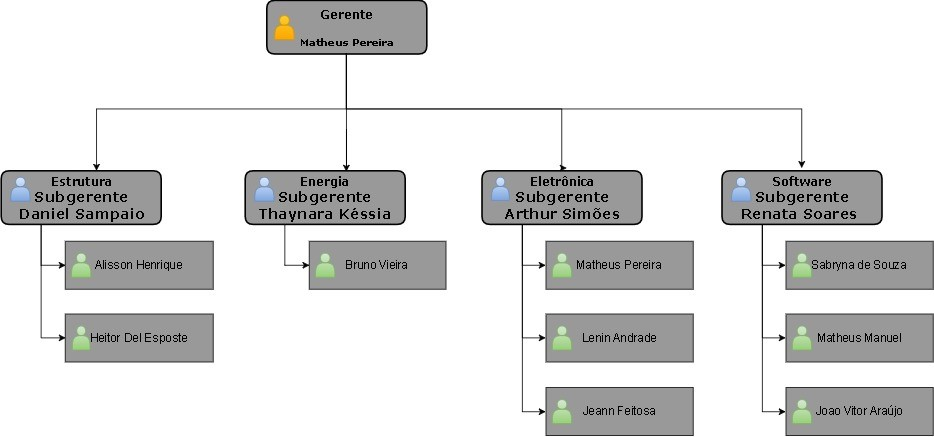
\includegraphics[scale=0.6]{figuras/Organograma}
	\captionof{figure}{Organograma do projeto.}
\end{center} 
    

    
    

